\documentclass{beamer}
\usepackage{physics}
\usepackage{wrapfig}
\usepackage{tikz}
\usepackage{circuitikz}
\graphicspath{{./image/}}
\usetheme{default}

\title{Le hack du millenaire?}
\subtitle{Et si on cassait RSA?}
\author{Kwame Yamgnane - kw@qwasar.io}
\institute{Qwasar Silicon Valley}

\begin{document}


\begin{frame}
        \titlepage
\end{frame}

\begin{frame}{Un processeur}{Transitors}
  \begin{columns}
    \begin{column}{0.5\textwidth}
      PNP
      \begin{circuitikz}
        \draw (0,0) node[pnp] (pnp) {};
      \end{circuitikz}
    \end{column}
    \begin{column}{0.5\textwidth}
      NPN
      \begin{circuitikz}
        \draw (0,0) node[npn] (npn) {};
      \end{circuitikz}
    \end{column}
  \end{columns}
\end{frame}

\begin{frame}{Un processeur}{Portes logiques = groupe de transistor / NAND}
  \begin{columns}
    \begin{column}{0.5\textwidth}
      \begin{circuitikz}
        \draw (0,2) node[npn](p1){};
        \draw (0,0) node[npn](p2){};
        \draw (-2,6) node[pnp](n1){};
        \draw (0,4) node[pnp](n2){};
        \draw (p1.E) -- (p2.C);
        \draw (p2.B) |- (n2.B);
        \draw (n1.B) |- (p1.B);
        \draw (n1.C) |- (n2.C);
        \draw (n2.C) to [short, *-o] ++(1.5,0);
        \draw (n1.E) to [short, -o] ++(3.5,0);
        \draw (n2.E) to [short, -*] ++(0,2);
        \draw (p2.E) to [short, -o] ++(1.5,0);
        \draw (p1.C) to (n2.C);
        \draw (-3.5,1.5) to[short, o-*] (-0.84,1.5);
        \draw (-3.5,4) to[short, o-*] (-2.84,4);
        \draw node [left] at (-3.5, 4) {A};
        \draw node [left] at (-3.5, 1.5) {B};
        \draw node [above] at (1.25, 6) {0};
        \draw node [below] at (1.25, 4) {out};
        \draw node [below] at (1.25, 0) {1};
      \end{circuitikz}
    \end{column}
    \begin{column}{0.25\textwidth}
      \begin{table}
        \begin{tabular}{r|c|c}
          A & B & Out  \\ \hline
          0 & 0 & 1 \\
          1 & 0 & 0 \\
          0 & 1 & 0 \\
          1 & 1 & 0 \\
        \end{tabular}
        \caption{NAND}
      \end{table}
    \end{column}
    \begin{column}{0.25\textwidth}
      \begin{circuitikz}
        \draw (0,0) node[nand port] {};
      \end{circuitikz}
    \end{column}
  \end{columns}
\end{frame}

\begin{frame}{Les portes logiques}{le binaire: l'addition (NDLR: je sais y a pas le retenu on fera a l'oral :D)}
  \begin{columns}
    \begin{column}{0.25\textwidth}
      \begin{table}
        \begin{tabular}{c|c}
          1 & 0 0 1  \\ \hline
          2 & 0 1 0  \\ \hline
          3 & 0 1 1  \\ \hline
          ... &...
        \end{tabular}
      \end{table}
      \begin{table}
        \begin{tabular}{r|c|c}
          A & B & Out  \\ \hline
          0 & 0 & 0 \\
          1 & 0 & 1 \\
          0 & 1 & 1 \\
          1 & 1 & 1 \\
        \end{tabular}
        \caption{OR}
      \end{table}
    \end{column}
    \begin{column}{0.75\textwidth}
      \begin{circuitikz}
        \draw (0,0) node[or port] {};
        \draw (0,2) node[or port] {};
        \draw (0,4) node[or port] {};
      \end{circuitikz}
    \end{column}
  \end{columns}
\end{frame}

\begin{frame}{Qui veut gagner 1 million ?}{P = NP}
  \begin{columns}
    \begin{column}{0.5\textwidth}
      \begin{itemize}
      \item Algorithmes compliqu\'{e}s
        \color{red}
      \item Algorithmes NP : Compliqu\'{e}s \`a executer, facile \`a r\'esoudre
        \color{blue}
      \item Algorithmes P : faciles \`a executer et \`a resoudre
      \end{itemize}
    \end{column}
  
    \begin{column}{0.5\textwidth}
      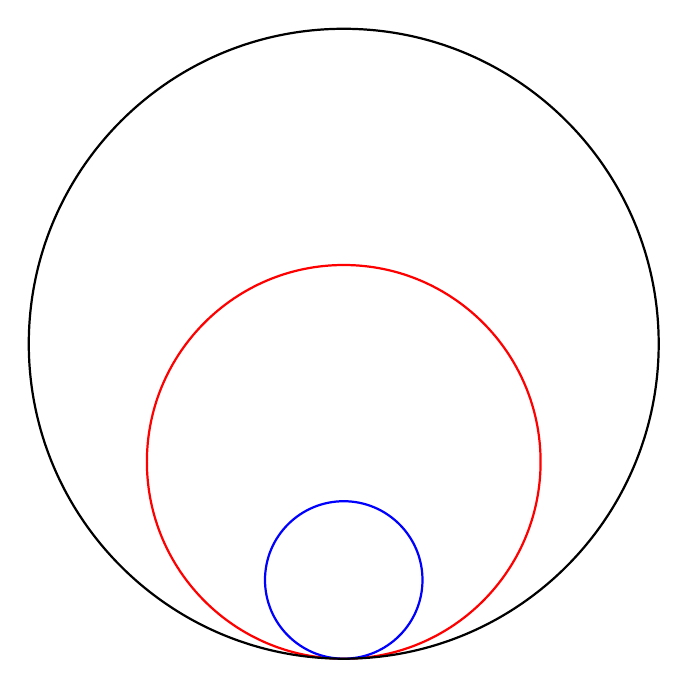
\begin{tikzpicture}
        \draw[thick, red] (2,2) circle (2.5cm);
        \draw[thick, blue] (2,0.5) circle (1cm);
        \draw[thick] (2,3.5) circle (4cm);
      \end{tikzpicture}
    \end{column}
  \end{columns}
\end{frame}

\begin{frame}{Quelques bases}{Exemple}
  \begin{columns}
    \begin{column}{0.5\textwidth}
      \begin{itemize}
      \item Trouver les facteurs premiers de $82661 \leftarrow NP$
      \item $41x43x47 = 82661 \leftarrow P$
      \end{itemize}
    \end{column}
    
    \begin{column}{0.5\textwidth}
      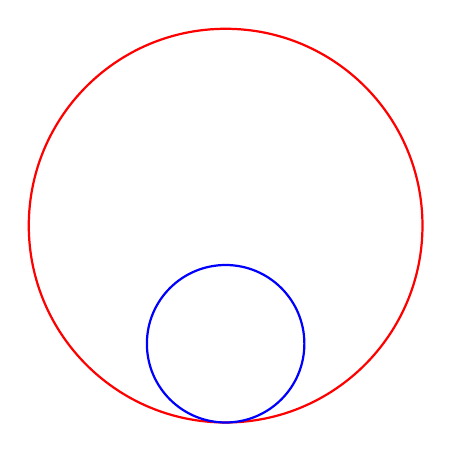
\begin{tikzpicture}
        \draw[thick, red] (2,2) circle (2.5cm);
        \draw[thick, blue] (2,0.5) circle (1cm);
      \end{tikzpicture}
    \end{column}
  \end{columns}
\end{frame}

\begin{frame}{Quelques bases}{choix des algorithmes de cryptographie}
  \begin{columns}
    \begin{column}{0.5\textwidth}
      Les algorithmes de crypto sont NP
    \end{column}
    
    \begin{column}{0.5\textwidth}
      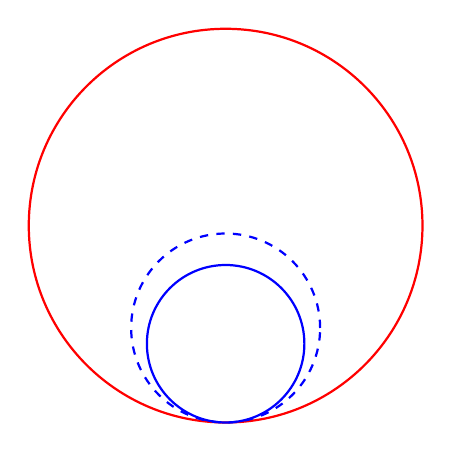
\begin{tikzpicture}
        \draw[thick, red] (2,2) circle (2.5cm);
        \draw[thick, blue, dashed] (2,0.70) circle (1.2cm);
        \draw[thick, blue] (2,0.5) circle (1cm);
      \end{tikzpicture}
    \end{column}
  \end{columns}
\end{frame}

\begin{frame}{Quelques bases}{La m\'{e}canique quantique}
  \begin{center}
    \begin{tabular}{ c c c }
      Le tout petit & \`{A} l'echelle humaine  & \`{A} partir de 1 \(M_\odot\) \\
      (niveau Atom) & & \\
      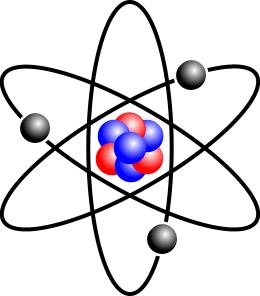
\includegraphics[height=2cm]{Atome_lithium_rutherford.png} & 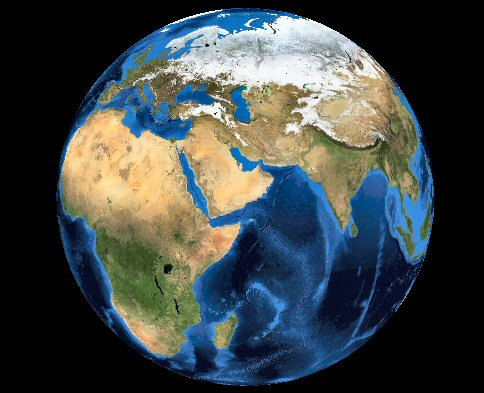
\includegraphics[height=2cm]{TerreWorldWind.jpg} & 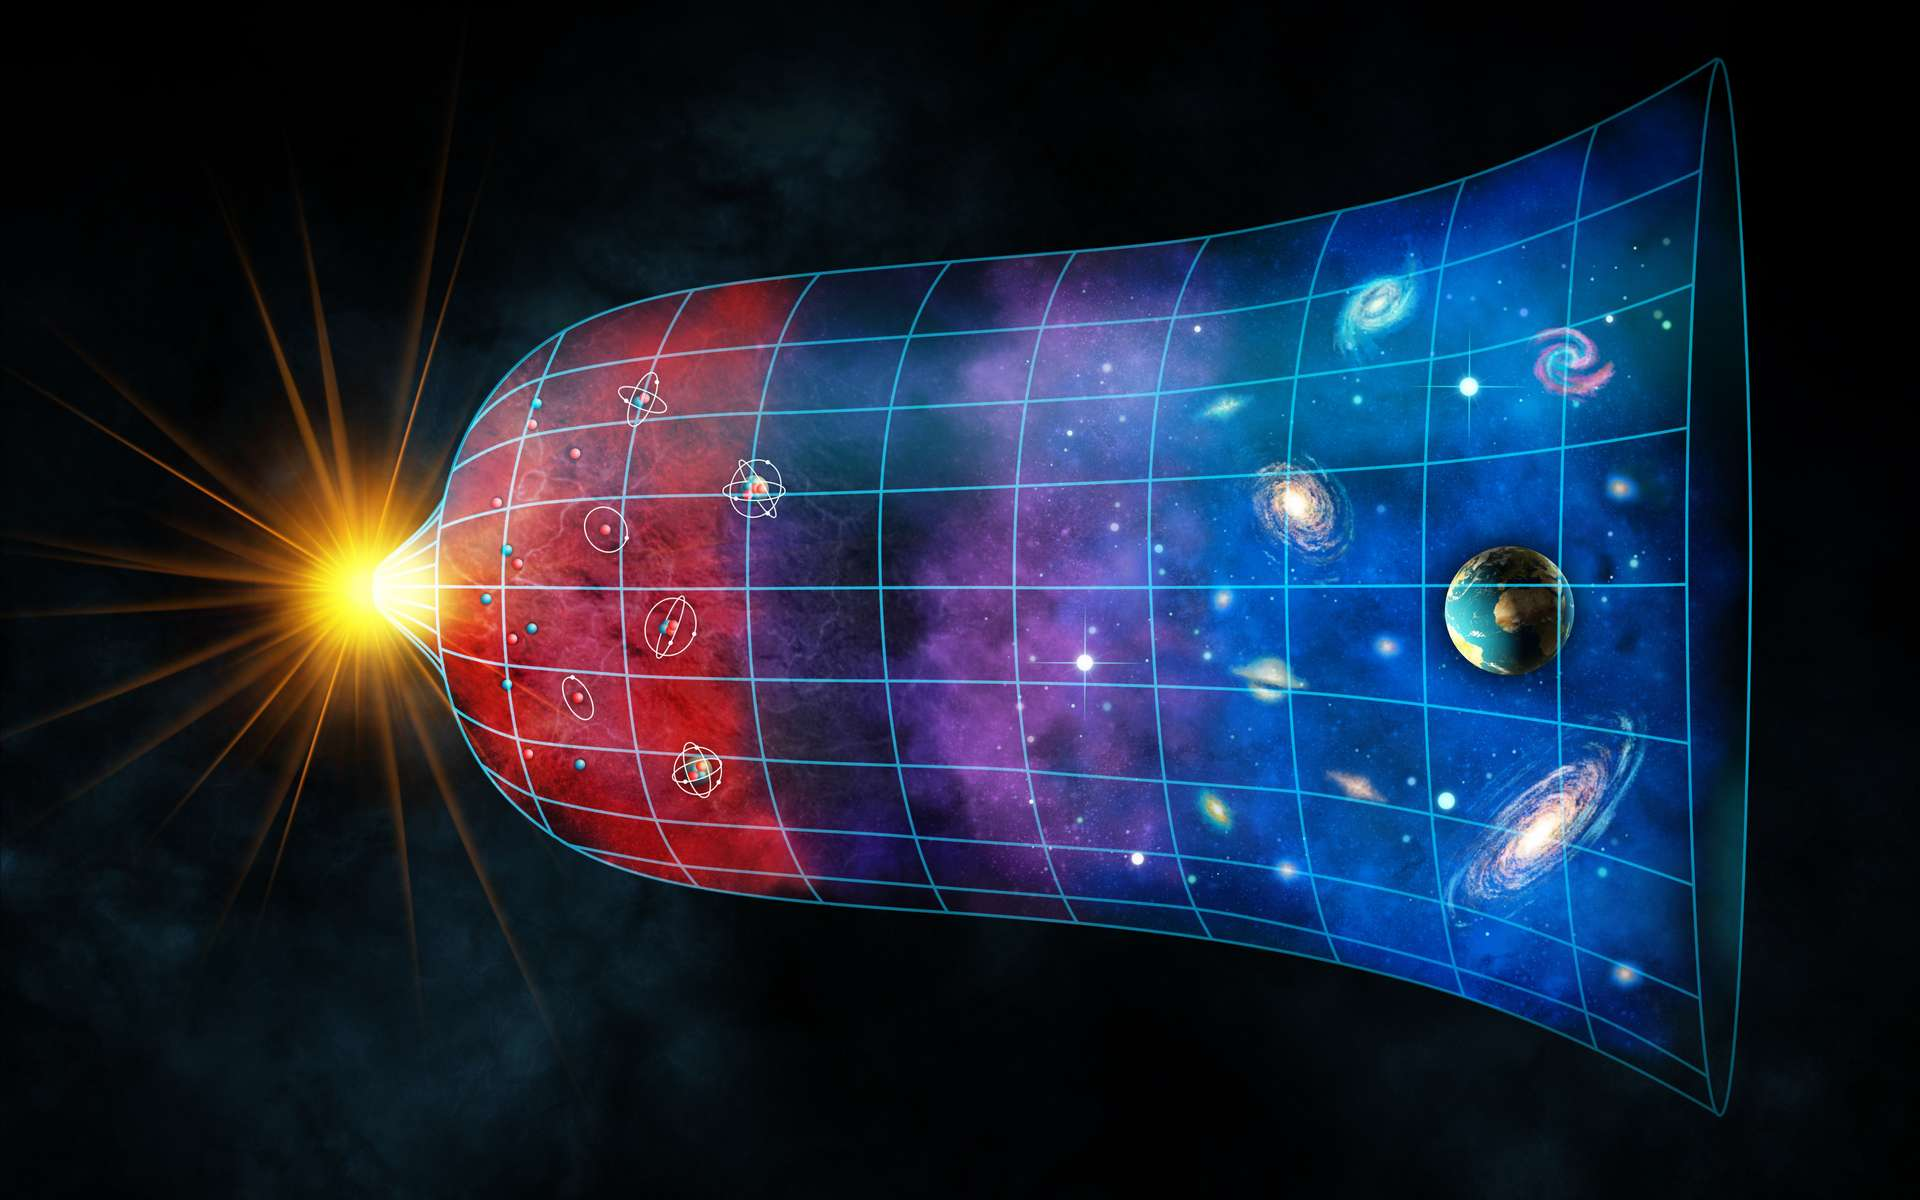
\includegraphics[height=2cm]{04-965413833409_COI.jpeg}\\
      Mecanique Quantique & Newton & Relativite generale \\
       &  & Newton Etendu \\
    \end{tabular}
  \end{center}
\end{frame}

\begin{frame}{Superposition Quantique}{``je suis inombrable''}
  \begin{center}
    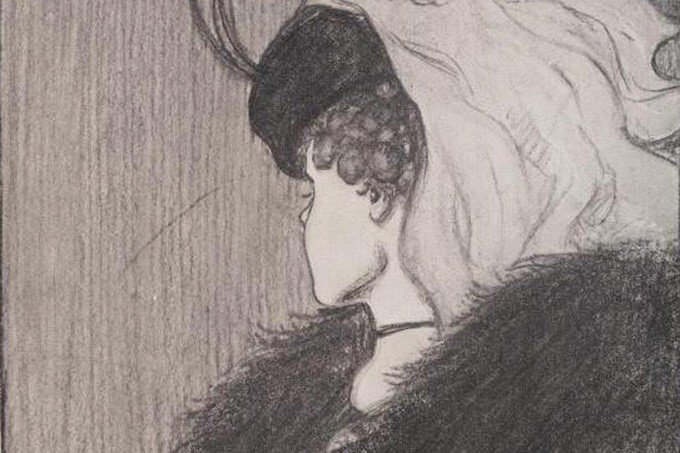
\includegraphics[width=9cm]{3604843-inline.jpg}\\
    \vspace{0.5cm}
    $\ket{\Psi} = a \ket{Jeune} + b \ket{Agee}$ 
  \end{center}
\end{frame}

\begin{frame}{Intrication Quantique}{``L'espace et le temps n'existent pas''}
  \begin{center}
        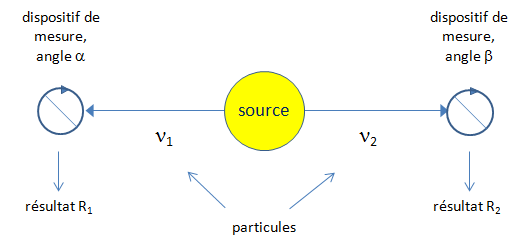
\includegraphics[width=9cm]{intrication.png}\\
    \vspace{0.5cm}
    $\ket{\Psi(v1, v2)} = \frac{1}{\sqrt{2}}(\ket{\Psi(\uparrow\downarrow)} - \ket{\Psi(\downarrow\uparrow)})$
  \end{center}
\end{frame}

%\begin{frame}
%\end{frame}

\begin{frame}
        Merci !
\end{frame}

\begin{frame}{Exhibit}{Les conferences d'Alain Aspect}

\end{frame}

\begin{frame}{Exhibit}{La chaine youtue de David Louarpe Science Etonnante}
  \begin{description}
  \item \href{https://www.youtube.com/watch?v=Rj3jTw2DxXQ&t=3s}{La mécanique quantique en 7 idées}
  \item \href{https://www.youtube.com/watch?v=5R6k2mEacZo&t=8s}{L'intrication quantique}
  \item \href{https://www.youtube.com/watch?v=hB1kmGzpIrw}{Les expériences d'Alain ASPECT}
  \item \href{https://www.youtube.com/watch?v=OeZ_63iKPho&t=556s}{Alain Aspect : Interview complète}
  \item \href{https://www.youtube.com/watch?v=hB1kmGzpIrw}{Le mystère des gâteaux quantiques}
  \item \href{https://www.youtube.com/watch?v=KaRd_eB2qOA}{La Suprématie Quantique de Google}
  \item \href{https://www.youtube.com/watch?v=AgtOCNCejQ8}{P = NP}
  \end{description}
\end{frame}

\begin{frame}{Exhibit}{Disclaimer}
  \begin{description}
  \item Speakable and Unspeakable in Quantum Mechanics: Collected Papers on Quantum Philosophy
  \item L'Impensable Hasard: Non-localité, téléportation et autres merveilles quantiques
  \item Introduction to Quantum Optics: From the Semi-classical Approach to Quantized Light
  \end{description}
\end{frame}

\end{document}
